\subsection{Minesweeper}
In the game of Minesweeper, there is an $m\times n$ board which has exactly $k$ mines hidden. The aim is to ``clear'' the board by clicking on cells with no mine and avoiding clicking on any mine. By clicking on a cell with no mine, the player gets the number of neighbouring mines of that cell by the below rule
\begin{itemize}	
	\item If the cell $c$ is not at the boundary (\ref{fig:minecnb}) then it is the number of mines in a $3\times3$ square with that centre $c$.
	\item If the cell $c$ is at the boundary (\ref{fig:minecb1}, \ref{fig:minecb1}) even then $c$ cell is considered as the centre of $3\times3$ square; but, only some of the cells of the constructed square will lie inside the board.
\end{itemize}
\begin{figure}[H]
	\centering
	\begin{subfigure}[t]{0.25\linewidth}
		\centering
		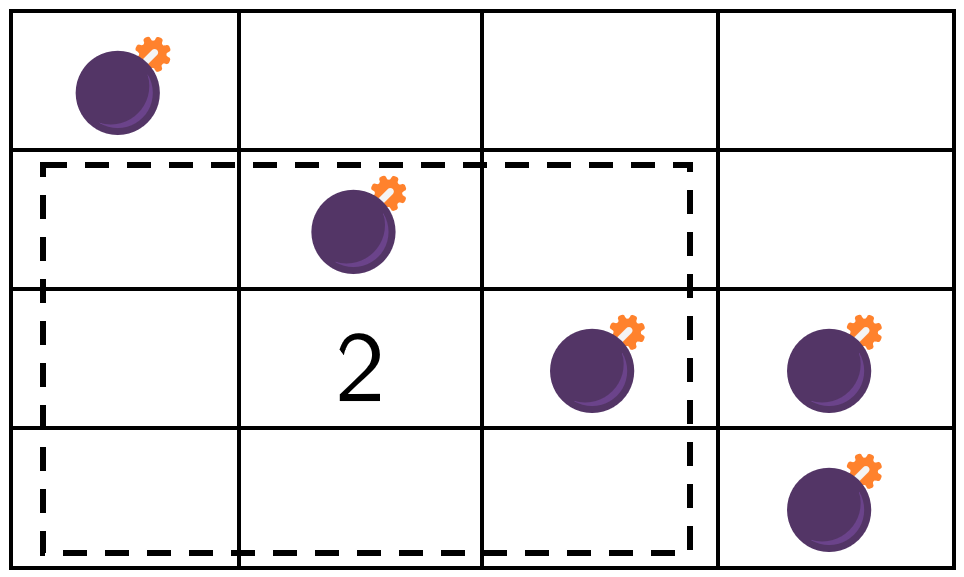
\includegraphics[height = 0.528\textwidth]{Minesweeper/middle.png}
		\caption{Cell is not at the boundary}
		\label{fig:minecnb}
	\end{subfigure}
	\begin{subfigure}[t]{0.22\linewidth}
		\centering
		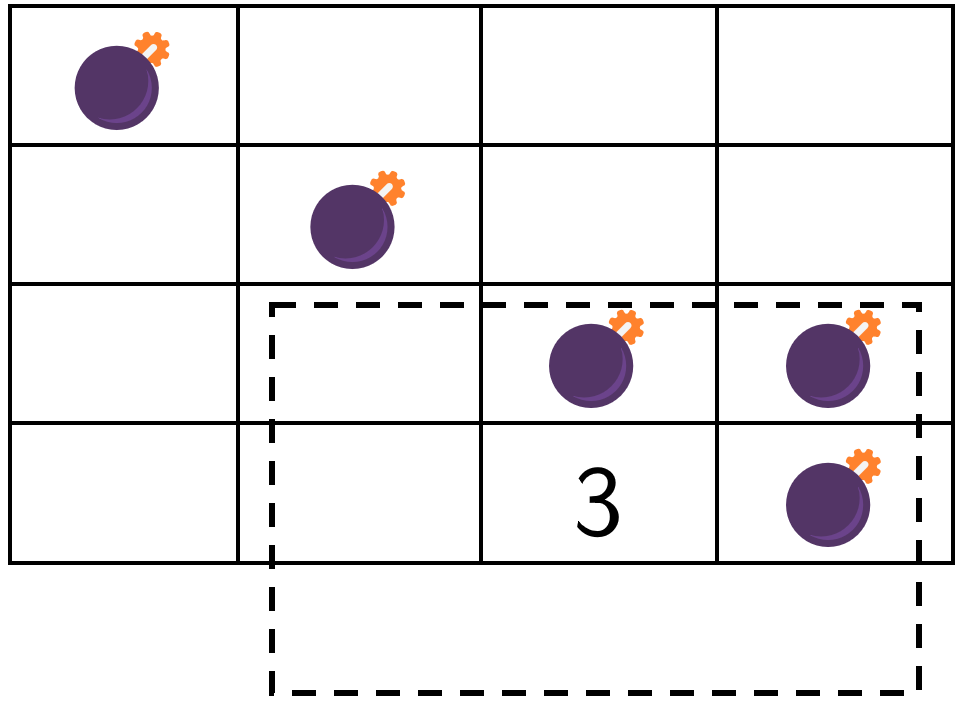
\includegraphics[height = 0.6\textwidth]{Minesweeper/bottom.png}
		\caption{Cell is at the boundary}
		\label{fig:minecb1}
	\end{subfigure}
	\begin{subfigure}[t]{0.22\linewidth}
		\centering
		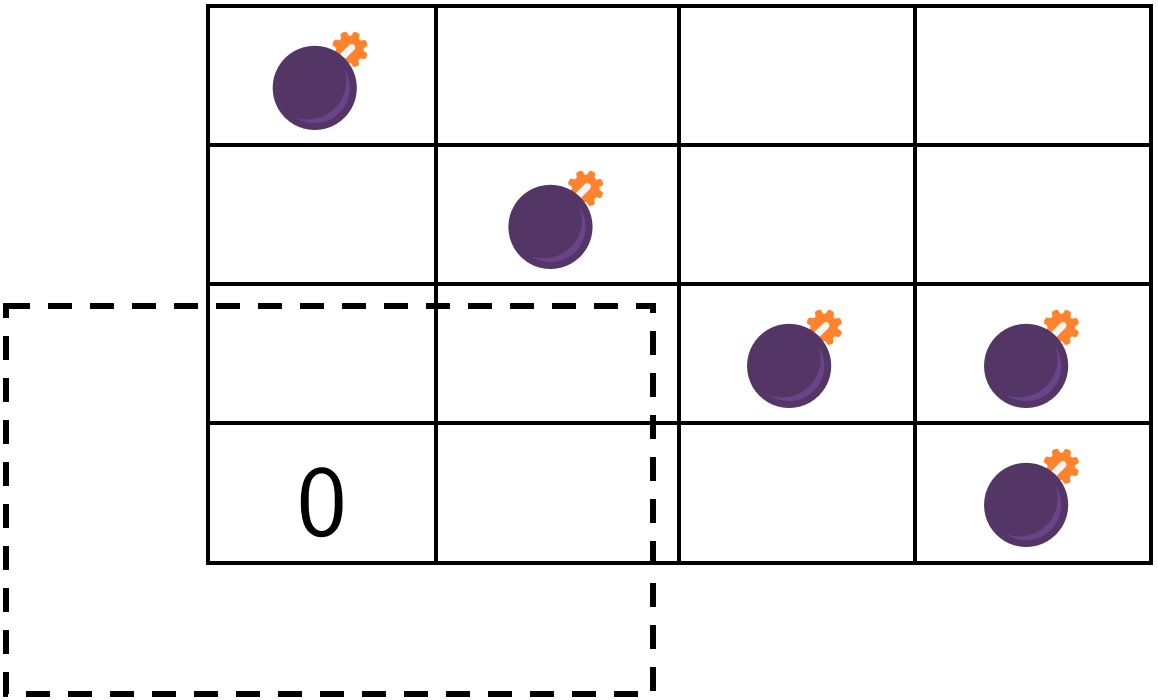
\includegraphics[height = 0.6\textwidth]{Minesweeper/corner.png}
		\caption{Cell is at the boundary}
		\label{fig:minecb2}
	\end{subfigure}
	\begin{subfigure}[t]{0.22\linewidth}
		\centering
		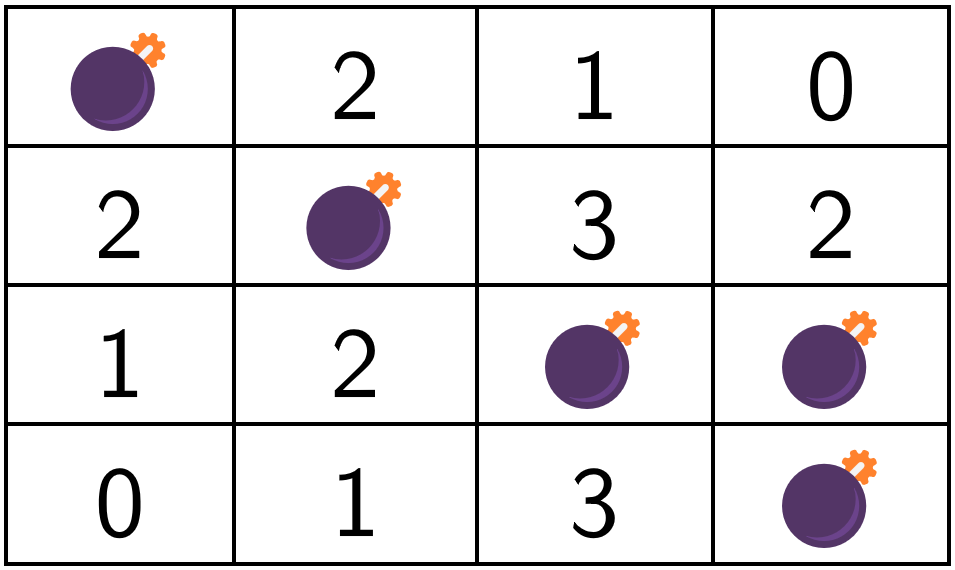
\includegraphics[height = 0.6\textwidth]{Minesweeper/explanation.png}
		\caption{Explanation for all cells}
		\label{fig:minee}
	\end{subfigure}
	\caption{Minesweeper -- Explanation}
\end{figure}
\vspace{-2em}
\textbf{Problem Statement:}\\
Calculate the neighbour count for all cells except at the mines where you have to output the character `M'.% in place of a number.
\begin{testcasesMore}
	{%$t$ \hfill(number of test cases, an integer)\\
	$m\ n$\hfill(space seperated integer pair corresponding to number of rows and columns)\\$k\quad x_1\ y_1\ \quad\cdots\quad x_{k}\ y_{k}$ \hfill($2k+1$ space seperated integers corresponding to number of mines and the $x,y$ co-ordinates of all mines (1-indexed))}
	%These numbers correspond to (number of rows, columns, mines, all co-ordinates of mine (2D, 1-indexed)).}
	{$m\times n$ matrix $A$, where $a_{ij}=\begin{cases}
		\text{`M'}& \text{if there is a mine at $(i,j)$} \\
		\text{number of neighbouring mines of the cell $(i,j)$} & \text{otherwise}
	\end{cases}$}
	{$1 \leq m,n \leq 50$, $1 \leq k \leq m\times n$\\$1 \leq x \leq m$, $1 \leq y \leq n$\\$0 \leq a_{ij} \leq 8$ or $a_{ij}=$ `M'.}%\hfill()
	{4 4\\5\qquad1 1 \quad2 2 \quad3 3\quad3 4\quad4 4}
	{M 2 1 0\\	2 M 3 2 \\	1 2 M M \\	0 1 3 M}
	{https://github.com/paramrathour/CS-101/tree/main/Test Cases/Minesweeper/Input}
	{https://github.com/paramrathour/CS-101/tree/main/Test Cases/Minesweeper/Output}
	{https://github.com/paramrathour/CS-101/tree/main/Starter Codes/Minesweeper.cpp}
\end{testcasesMore}
\begin{note}
	Try implementing the complete minesweeper game :)
\end{note}